
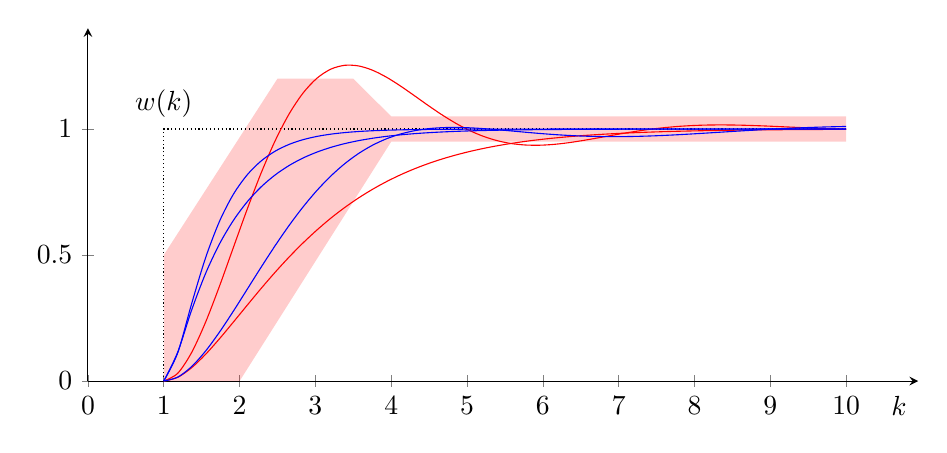
\begin{tikzpicture}
\pgfplotsset{width=1.0\columnwidth,height=0.5\columnwidth}



\begin{axis}[
       xmin=0,
       xmax=10.95,
       ymin=0,
       ymax=1.4,
       axis x line = bottom,
       axis y line = left,
]

\draw[draw=none,fill=red,opacity=0.2]
    (axis cs:1,0)     -- (axis cs:1,0.5)
 -- (axis cs:2.5,1.2)   -- (axis cs: 3.5,1.2)
 -- (axis cs:4,1.05)  -- (axis cs: 10,1.05)
 -- (axis cs:10,0.95) -- (axis cs: 4,0.95)
 -- (axis cs:2,0)
 -- cycle;

\addplot[black,densely dotted]
    coordinates{(1,0)(1,1)(10,1)};

\addplot[domain=1:10,samples=50,smooth,red]
    {1+(exp(-(14*(x-1))/25)*(-25*cos(deg(7*sqrt(21)*(x-1))/25)
            -(50*sin(deg(7*sqrt(21)*(x-1))/25))/sqrt(21)))/25};
\addplot[domain=1:10,samples=50,smooth,red]
    {1-exp(-(x-1)))-(x-1)*exp(-(x-1)))};

\addplot[domain=1:10,samples=50,smooth,blue]
    {1-(8*exp(-(5*(x-1))/4))/7+exp(-10*(x-1))/7};
\addplot[domain=1:10,samples=50,smooth,blue]
    {1-(5*exp(-2*(x-1)))/3+(2*exp(-5*(x-1)))/3};
\addplot[domain=1:10,samples=50,smooth,blue]
    {exp(-(x-1)/2)*(-cos(deg((sqrt(3)*(x-1))/2))
         -sin(deg((sqrt(3)*(x-1))/2)/sqrt(3)))+1};

\node[black] at (axis cs:1,1.1){$w(k)$};

\end{axis}

\node[black] at (10.3,-0.32){$k$};


\end{tikzpicture}
